%%%%%%%%%%%%%%%%%%%%%%%%%%%%%%%%%%%%%%%%%%%%%%%%%%%%%%%%%%%%%%%
%
% Welcome to Overleaf --- just edit your LaTeX on the left,
% and we'll compile it for you on the right. If you open the
% 'Share' menu, you can invite other users to edit at the same
% time. See www.overleaf.com/learn for more info. Enjoy!
%
%%%%%%%%%%%%%%%%%%%%%%%%%%%%%%%%%%%%%%%%%%%%%%%%%%%%%%%%%%%%%%%



% Inbuilt themes in beamer
\documentclass{beamer}

% Theme choice:
\usetheme{CambridgeUS}
\setbeamertemplate{caption}[numbered]{}

\usepackage{enumitem}
\usepackage{tfrupee}
\usepackage{amsmath}
\usepackage{amssymb}
\usepackage{gensymb}
\usepackage{graphicx}
\usepackage{txfonts}

\def\inputGnumericTable{}

\usepackage[latin1]{inputenc}                                 
\usepackage{color}                                            
\usepackage{array}                                            
\usepackage{longtable}                                        
\usepackage{calc}                                             
\usepackage{multirow}                                         
\usepackage{hhline}                                           
\usepackage{ifthen}
\usepackage{caption} 
\captionsetup[table]{skip=3pt}  
\providecommand{\pr}[1]{\ensuremath{\Pr\left(#1\right)}}
\providecommand{\brak}[1]{\ensuremath{\left(#1\right)}}
\providecommand{\cbrak}[1]{\ensuremath{\left\{#1\right\}}}
\renewcommand{\thetable}{\arabic{table}}
\providecommand{\abs}[1]{\left\vert#1\right\vert}

\let\vec\mathbf


% Title page details: 
\title{AI1110 : Probability and Random Variables}
\subtitle{Assignment 6} 
\author{Mannem Charan(AI21BTECH11019)}
\date{\today}


\begin{document}
% Title page frame
\begin{frame}
    \titlepage 
\end{frame}


% Outline frame
\begin{frame}{Outline}
    \tableofcontents
\end{frame}


% Lists frame
\section{Question}
\begin{frame}{Question}
 The random variable $x$ is uniform in the interval $\brak{-2c,2c}$. Find and sketch $f_{y}\brak{y}$ and $F_{y}\brak{y}$ if $y = g\brak{x}$ and $g\brak{x}$ is the function in Fig. 5-3.
\end{frame}

\section{Solution}
\subsection{Calculation}
\begin{frame}{Solution:Calculation} Given that, random variable $x$ is uniformly distributed in interval $\brak{-2c,2c}$ . So we can write that, the probability density function 
               \begin{align}
                        f_{x}\brak{x} &= \frac{1}{2c - \brak{-2c}}\\
                                            &= \frac{1}{4c}
               \end{align}
       So for $ x \in \brak{-2c,2c} $ , the probability distribution function $F_{x}\brak{x}$ can be calculated as,
               \begin{align}
                           F_{x}\brak{x} &= \int_{-2c}^{x} f_x\brak{x}dx\\
                                                &= \int_{-2c}^{x} \frac{1}{4c}dx\\
               \end{align}
\end{frame}
\begin{frame}
                \begin{align}             &= \frac{1}{4c}\int_{-2c}^{x}dx\\
                                                &= \frac{1}{4c}\brak{x + 2c}\\
                                                &= \frac{x+2c}{4c}
                \end{align}
            Since $x$ is distributed from -2c to 2c, we can write
                 \begin{equation*}
                                 F_{x}\brak{x} = \begin{cases}
                                                          0  &, x \leq -2c \\
                                                         \frac{x+2c}{4c} &, \abs{x} < 2c \\
                                                         1  & , x \geq 2c
                                                        \end{cases}
                 \end{equation*}
\end{frame}
\begin{frame}
            Now given that random variable $y$ is
                      \begin{align}
                                 y = g\brak{x}= x^2
                       \end{align}                                 
               When $ y \geq 0 $ and $ y < 4c^2 \brak{because x \in \brak{-2c,2c}}$ we can write probability distribution function in $y$ as,
                     \begin{align}
                              F_{y}\brak{y} &= \pr{Y \leq y}\\
                                                   &= \pr{g\brak{x} \leq y}\\
                                                   &= \pr{x^2 \leq y}\\
                                                   &= \pr{-\sqrt{y} \leq x \leq \sqrt{y}} \\
                                                   & = \pr{ x \leq \sqrt{y}} - \pr{ x \leq -\sqrt{y}} \\
                                                   & = F_{x}\brak{\sqrt{y}} - F_{x}\brak{-\sqrt{y}} \\
                                                   & = \frac{\sqrt{y} +2c}{4c} - \frac{-\sqrt{y} +2c}{4c} \\
                                                   & = \frac{\sqrt{y}}{2c}
                      \end{align}
\end{frame}
\begin{frame}
               Now for $ y < 0 $ there are no values of $x$ such that $ x^2 < y $ . So,
                              \begin{align}
                                     F_{y}\brak{y} = \pr{\emptyset} = 0 \brak{y<0}
                               \end{align}
            Overall we can write that,
                      \begin{equation*}
                               F_{y}\brak{y} = \begin{cases}
                                                          0  &, y < 0 \\
                                                         \frac{\sqrt{y}}{2c} &, 0\leq y \leq 4c^2 \\
                                                         1  & , y > 4c^2
                                                        \end{cases}
                      \end{equation*}
\end{frame}
\begin{frame}
             The probability density function $f_{y}\brak{y}$ for $ 0 \leq y \leq 4c^2 $ can be calculated as ,
                     \begin{align}
                                  f_{y}\brak{y} &= \frac{dF_{y}\brak{y}}{dy}\\
                                                       &= \frac{d}{dy}\brak{\frac{\sqrt{y}}{2c}} \\
                                                       & = \frac{1}{4\sqrt{y}c}
                      \end{align}
The plot of $ F_{x}\brak{x} ,F_{y}\brak{y},f_{y}\brak{y}$ for $c=1$ is shown below,
\end{frame}
\subsection{Plot}
\begin{frame}{Solution:Plot}
\begin{figure}
    \centering
    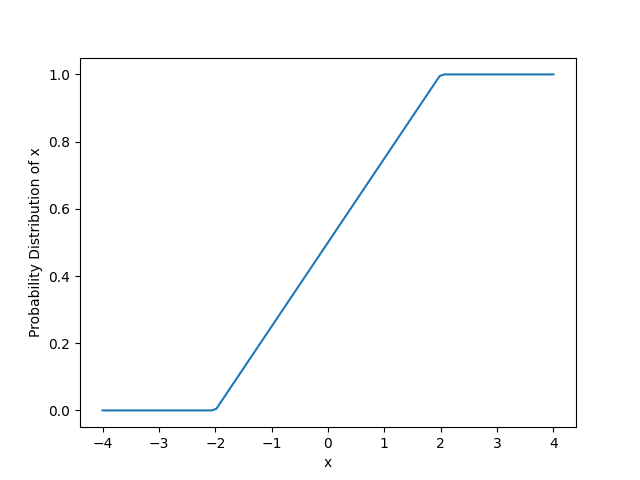
\includegraphics[width=9cm]{Prob_distribution_x.png}
    \caption{ }
    \label{Figure 1}
   \end{figure}
\end{frame}

\begin{frame}
\begin{figure}
    \centering
    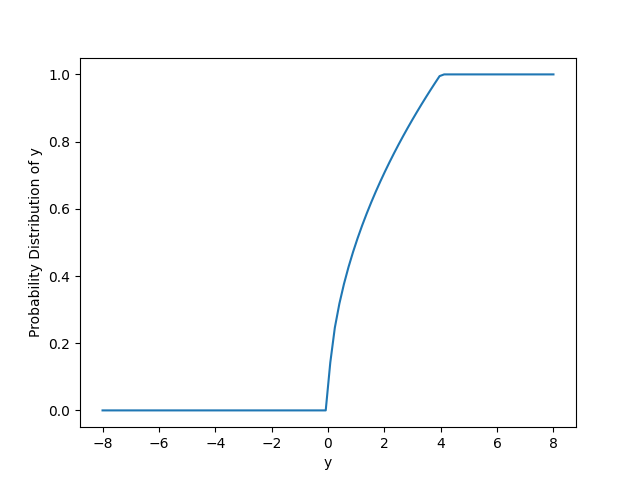
\includegraphics[width=10cm]{Prob_distribution_y.png}
    \caption{}
    \label{Figure 2}
\end{figure}
\end{frame}
\begin{frame}

  \begin{figure}
   \centering
    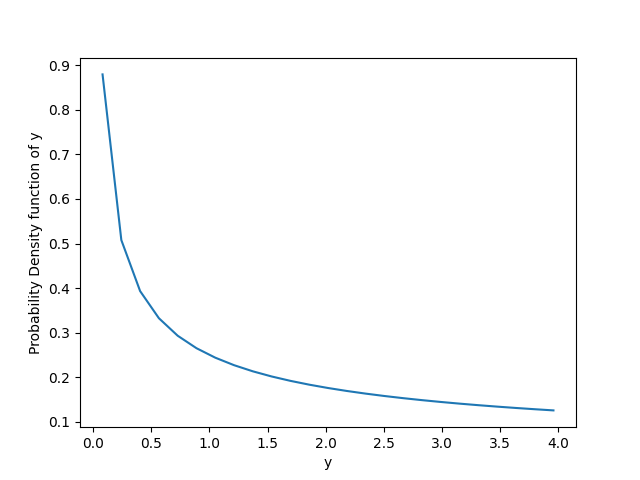
\includegraphics[width=10cm]{Prob_density.png}
   \caption{}
  \label{Figure 3}
  \end{figure}

\end{frame}
\end{document}
